% Digital Logic Report Template
% Created: 2020-01-10, John Miller

%==========================================================
%=========== Document Setup  ==============================

% Formatting defined by class file
\documentclass[11pt]{article}

% ---- Document formatting ----
\usepackage[margin=1in]{geometry}	% Narrower margins
\usepackage{booktabs}				% Nice formatting of tables
\usepackage{graphicx}				% Ability to include graphics

%\setlength\parindent{0pt}	% Do not indent first line of paragraphs 
\usepackage[parfill]{parskip}		% Line space b/w paragraphs
%	parfill option prevents last line of pgrph from being fully justified

% Parskip package adds too much space around titles, fix with this
\RequirePackage{titlesec}
\titlespacing\section{0pt}{8pt plus 4pt minus 2pt}{3pt plus 2pt minus 2pt}
\titlespacing\subsection{0pt}{4pt plus 4pt minus 2pt}{-2pt plus 2pt minus 2pt}
\titlespacing\subsubsection{0pt}{2pt plus 4pt minus 2pt}{-6pt plus 2pt minus 2pt}

% ---- Hyperlinks ----
\usepackage[colorlinks=true,urlcolor=blue]{hyperref}	% For URL's. Automatically links internal references.

% ---- Code listings ----
\usepackage{listings} 					% Nice code layout and inclusion
\usepackage[usenames,dvipsnames]{xcolor}	% Colors (needs to be defined before using colors)

% Define custom colors for listings
\definecolor{listinggray}{gray}{0.98}		% Listings background color
\definecolor{rulegray}{gray}{0.7}			% Listings rule/frame color

% Style for Verilog
\lstdefinestyle{Verilog}{
	language=Verilog,					% Verilog
	backgroundcolor=\color{listinggray},	% light gray background
	rulecolor=\color{blue}, 			% blue frame lines
	frame=tb,							% lines above & below
	linewidth=\columnwidth, 			% set line width
	basicstyle=\small\ttfamily,	% basic font style that is used for the code	
	breaklines=true, 					% allow breaking across columns/pages
	tabsize=3,							% set tab size
	commentstyle=\color{gray},	% comments in italic 
	stringstyle=\upshape,				% strings are printed in normal font
	showspaces=false,					% don't underscore spaces
}

% How to use: \Verilog[listing_options]{file}
\newcommand{\Verilog}[2][]{%
	\lstinputlisting[style=Verilog,#1]{#2}
}

\begin{document}

\title{ELC 2137 Lab 08: 4-digit Display}
\author{My Nguyen}

\maketitle

\section*{Summary}
This lab's purpose is to use parameter to create flexible, reusable module and use import modules to create modular design. First part is to create a mux2 module with uses parameter to generate mux2 module with different number of bit for input and output. Then, create mux4, and sseg4 module accordingly to the given schematic. Afterward, create a sseg4\_manual as a top-level module to do on-board testing. Finally, import basys3.sv and disp.sv file to do top-level simulation.

\section*{Table and Figure}
\begin{figure}[ht]
	\centering
	\includegraphics[width=\textwidth,trim=24cm 23cm 0.5cm 5cm,clip]{"mux2"}
	\caption{Mux2 ERT}
	\includegraphics[width=\textwidth,trim=24cm 23cm 0.5cm 5cm,clip]{"mux4"}
	\caption{Mux4 ERT}
	\includegraphics[width=\textwidth,trim=24cm 22cm 0.5cm 5cm,clip]{"an_decoder"}
	\caption{Anode Decoder ERT}
\end{figure}

\section*{Code}
\Verilog[firstline=23,caption=Mux2 Implementation]{../verilog_code/mux2.sv}
\Verilog[firstline=23,caption=Mux4 Implementation]{../verilog_code/mux4.sv}
\Verilog[firstline=23,caption=Anode Decoder Implementation]{../verilog_code/an_decoder.sv}
\Verilog[firstline=23,caption=Top Level Implementation]{../verilog_code/sseg4.sv}
\Verilog[firstline=23,caption=On-Board Implementation]{../verilog_code/sseg4_manual.sv}

\section*{Screenshot}
\begin{figure}[ht]
	\centering
	\includegraphics[width=12cm]{"board/step1"}
	\caption{1st Operation}
\end{figure}
\begin{figure}[ht]
	\centering
	\includegraphics[width=12cm]{"board/step2"}
	\caption{2nd Operation}
	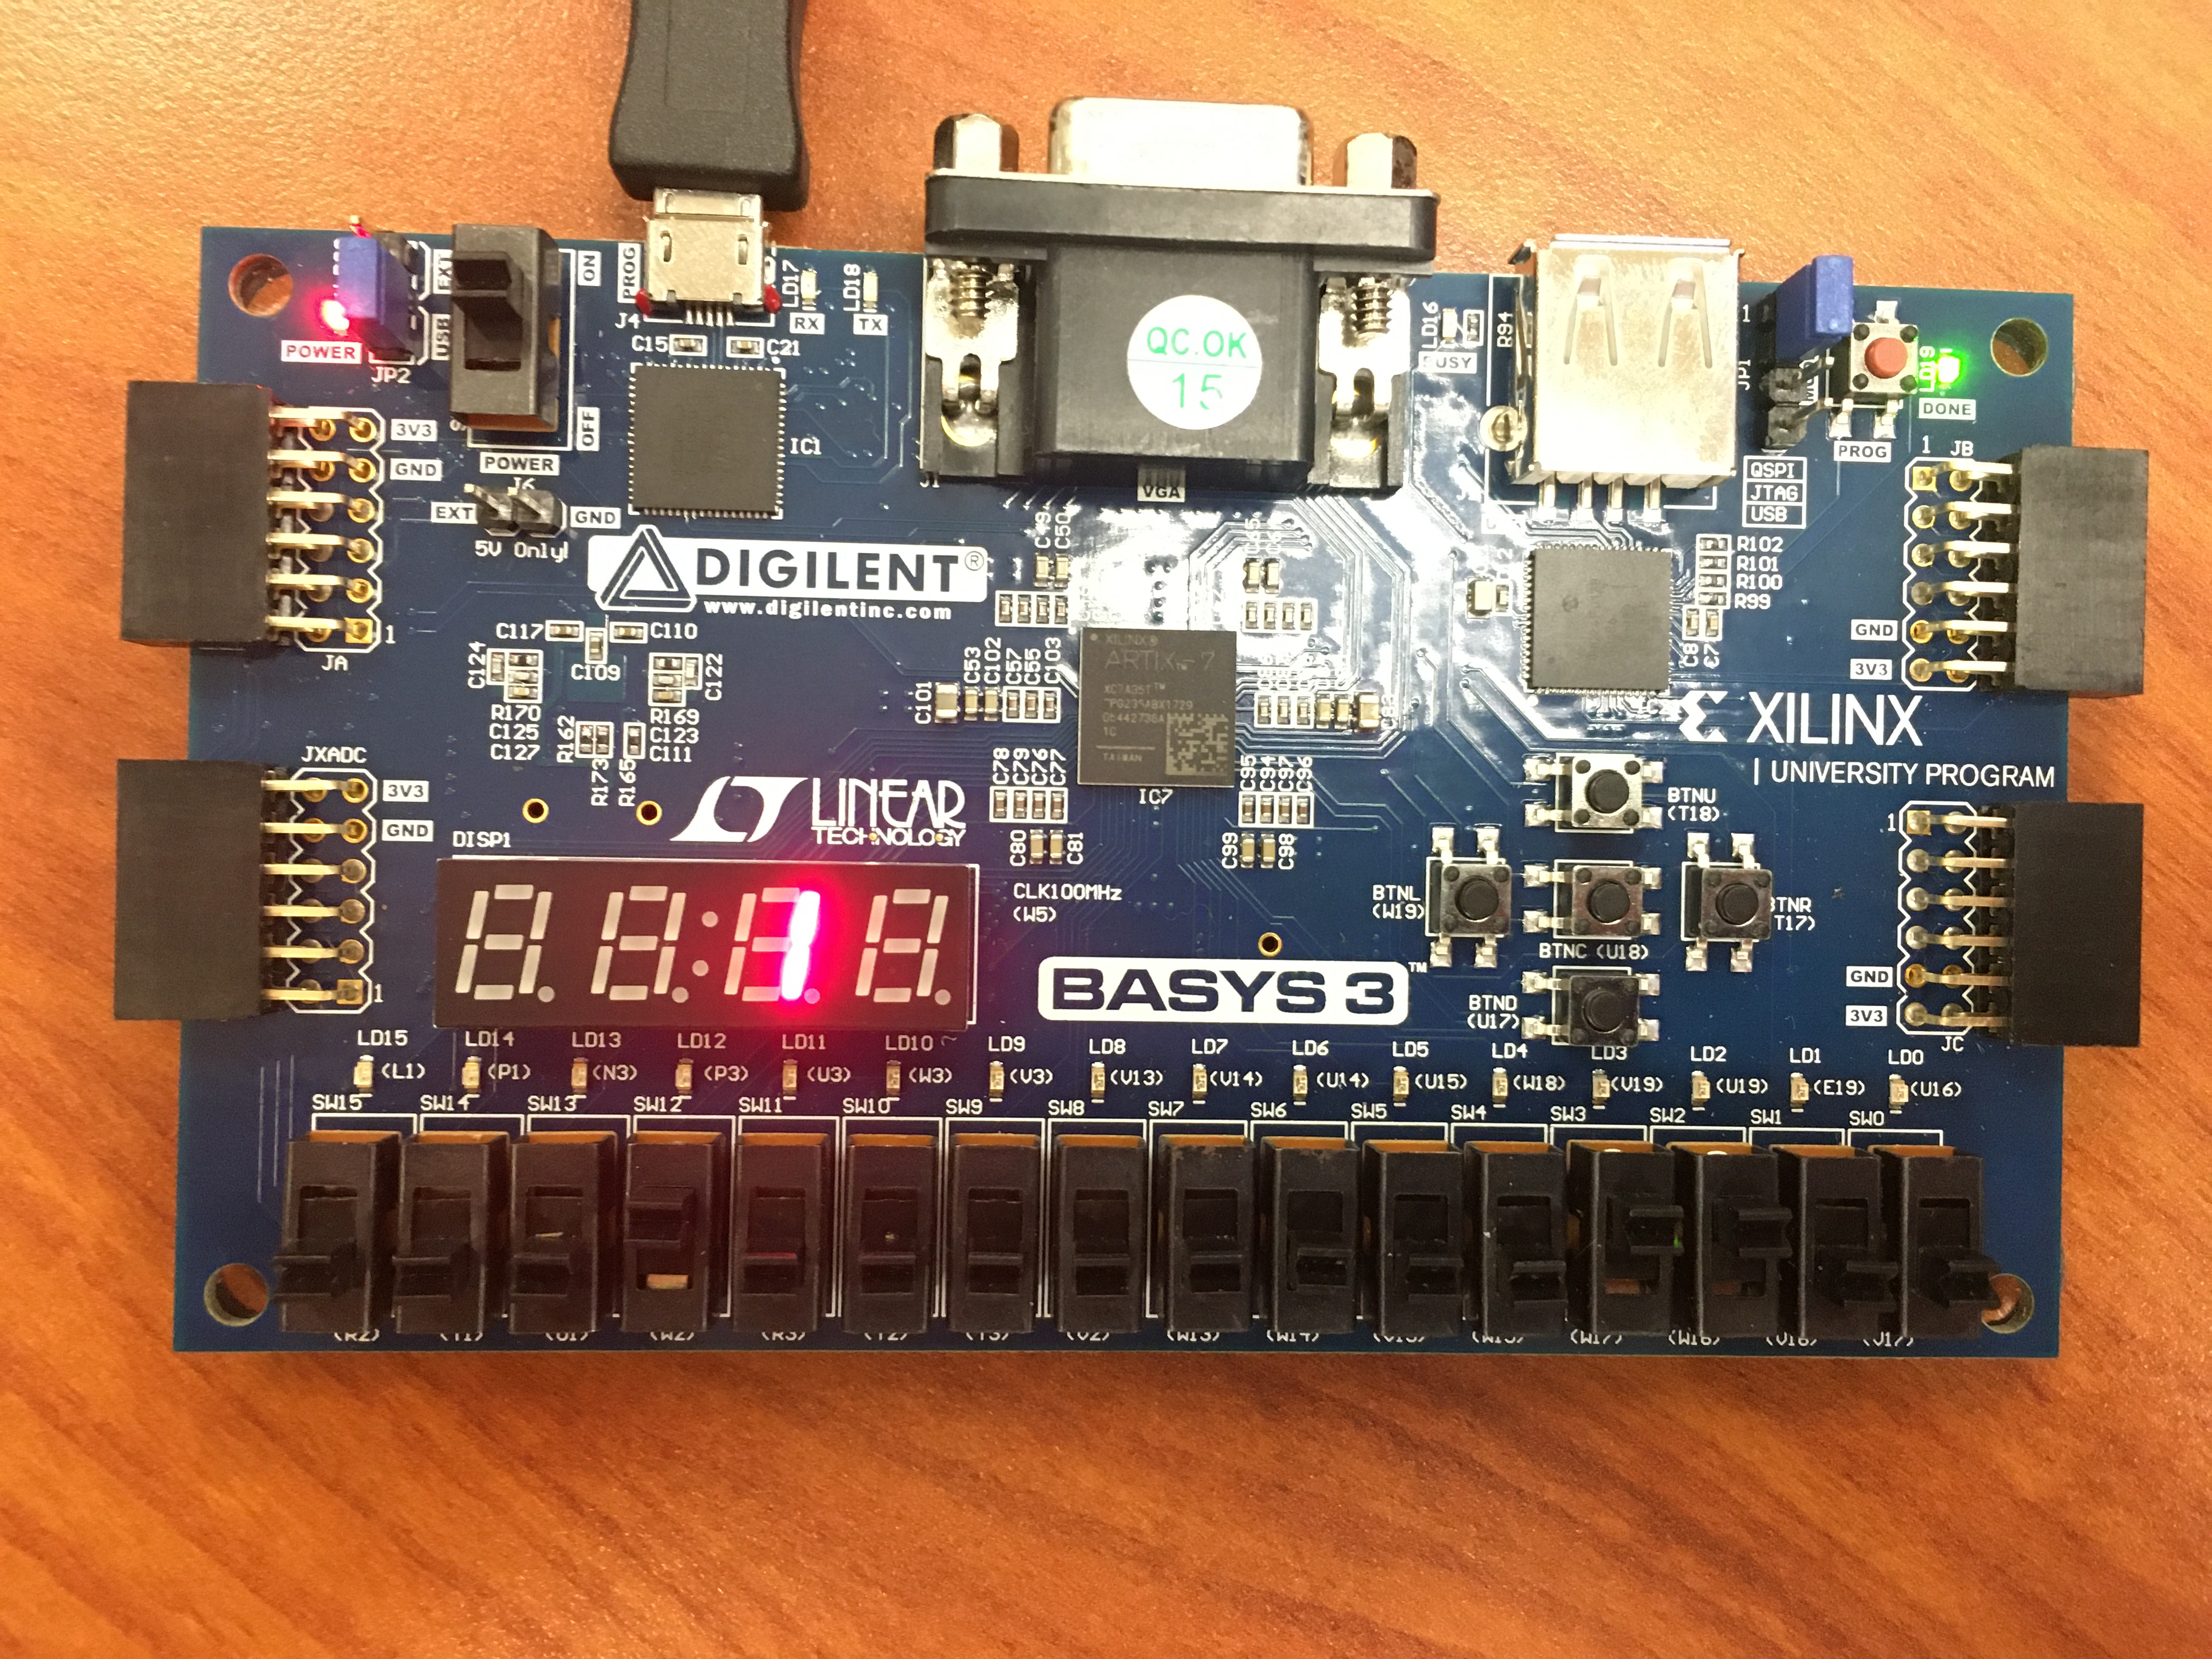
\includegraphics[width=12cm]{"board/step3}
	\caption{3rd Operation}
\end{figure}
\begin{figure}[ht]
	\centering
	\includegraphics[width=12cm]{"board/step4"}
	\caption{4th Operation}
	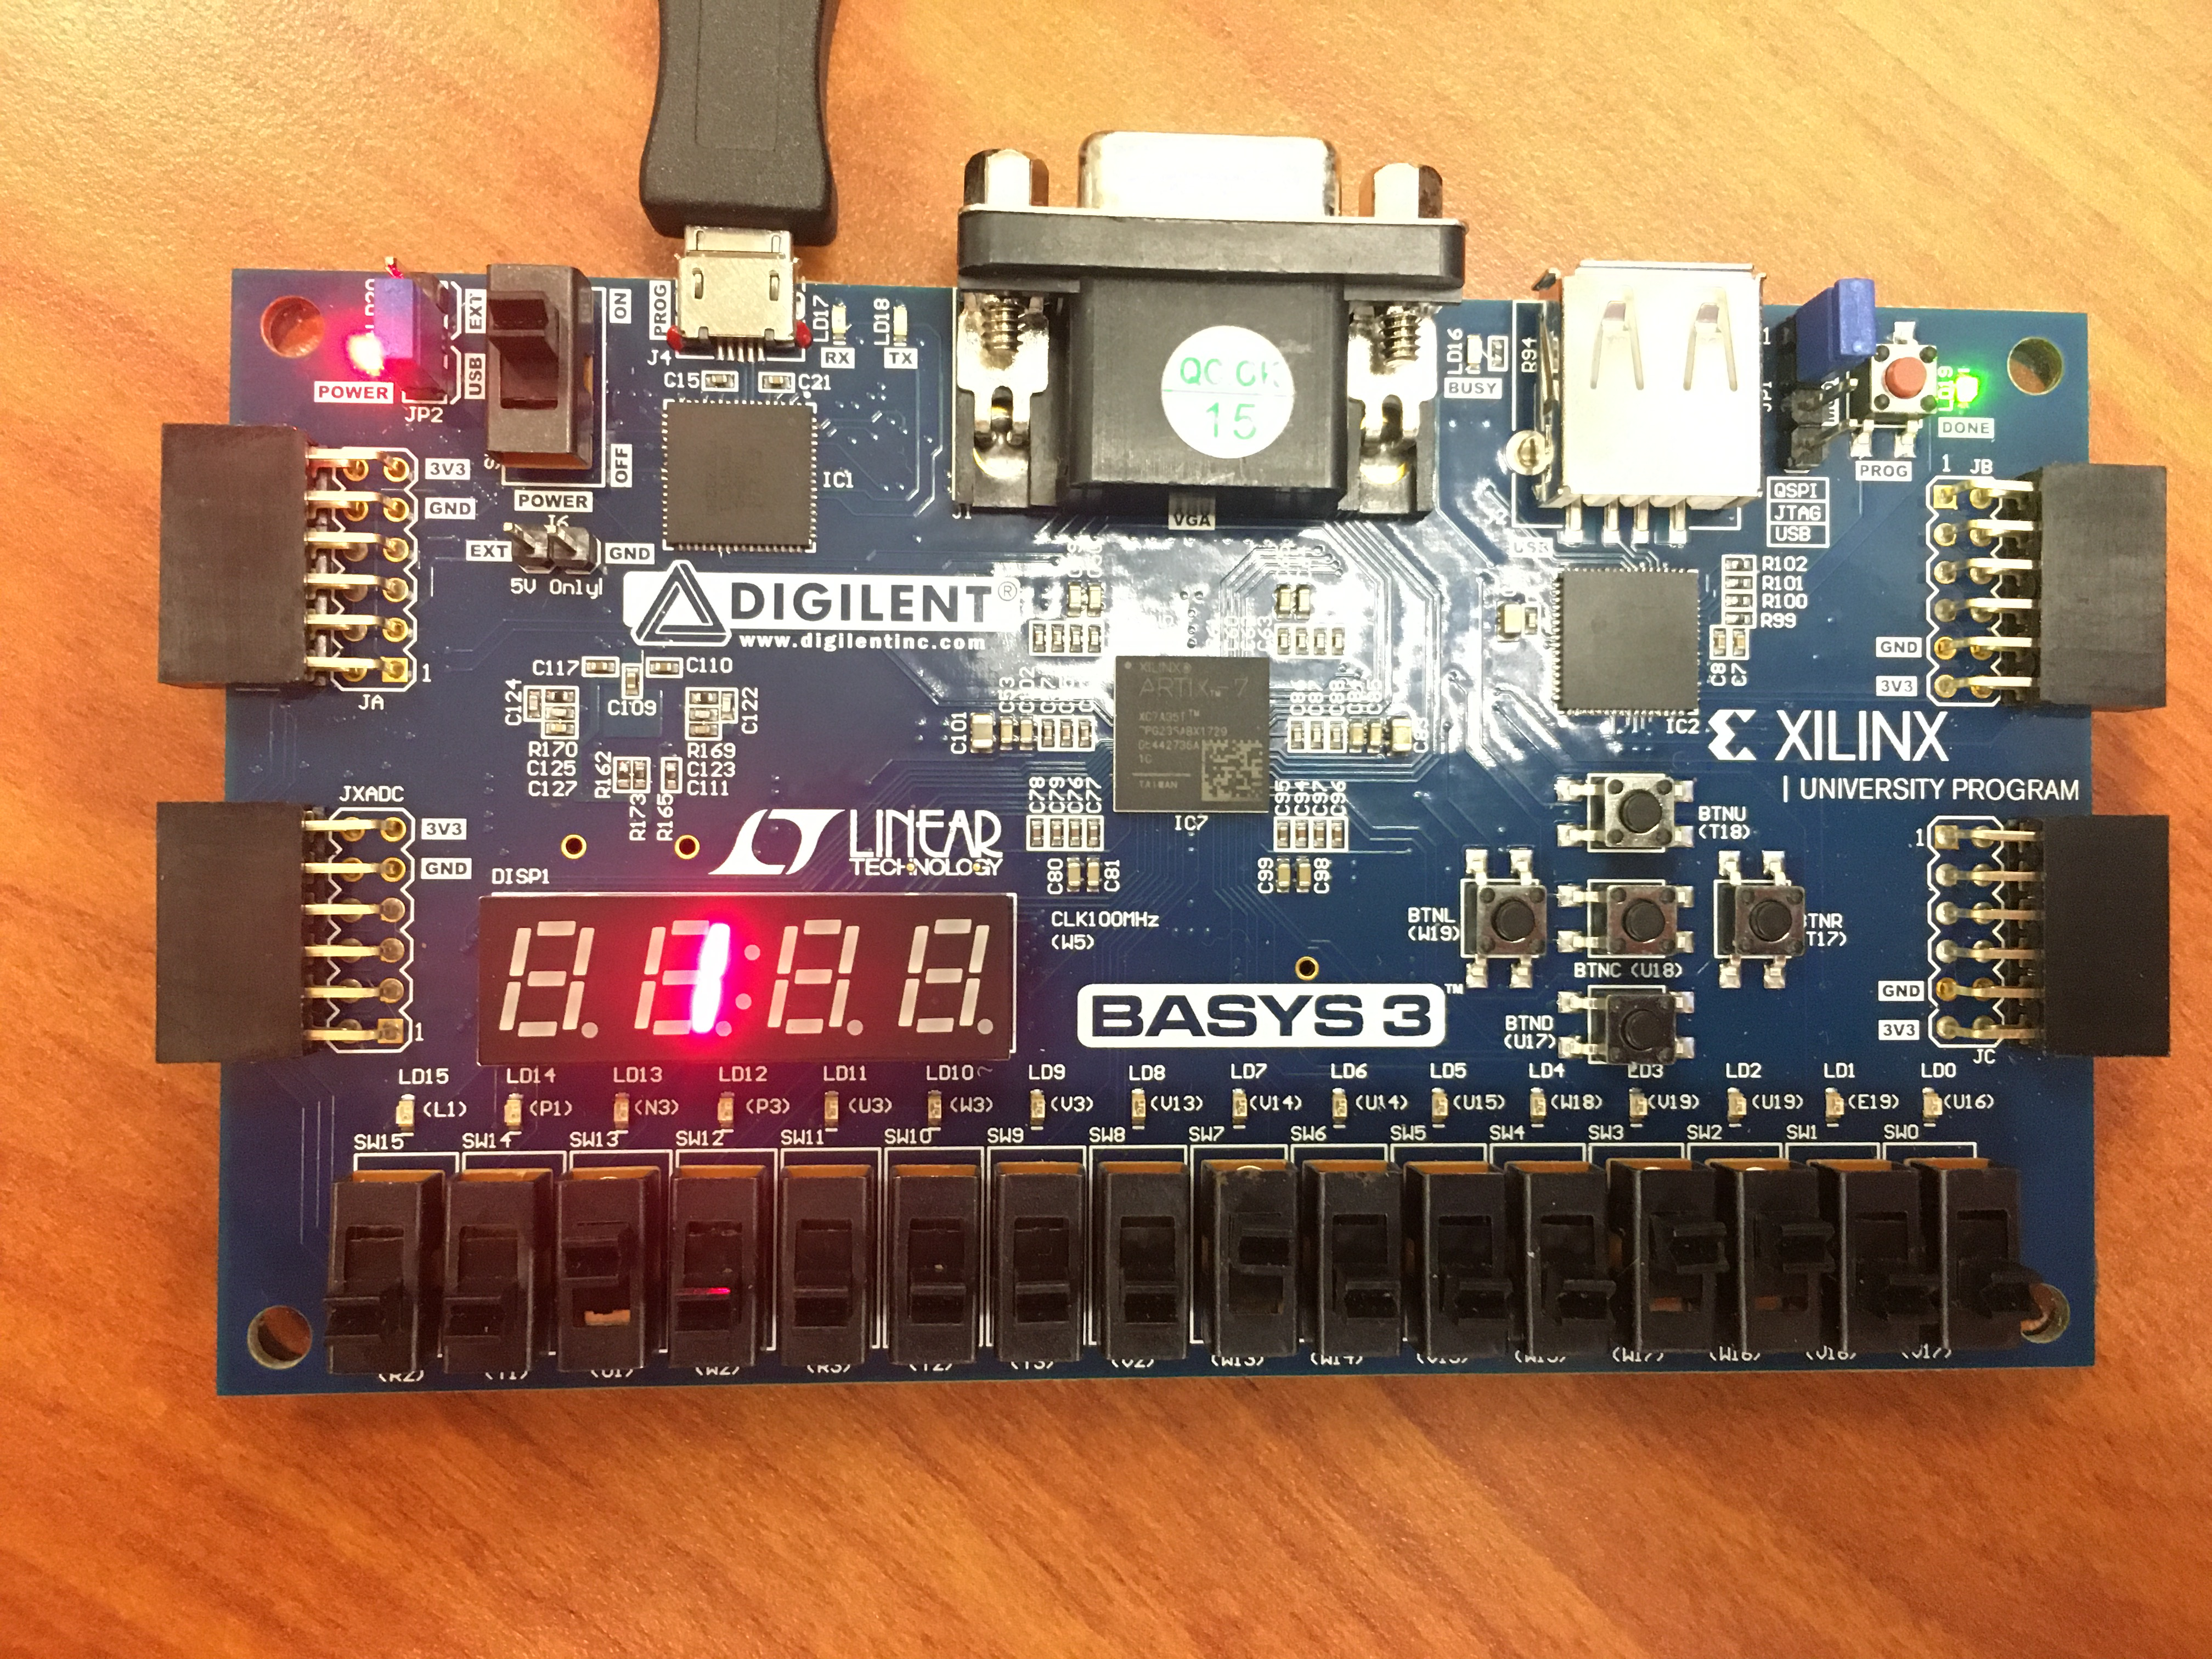
\includegraphics[width=12cm]{"board/step5}
	\caption{5th Operation}
\end{figure}
\begin{figure}[ht]
	\centering
	\includegraphics[width=12cm]{"board/step6"}
	\caption{6th Operation}
	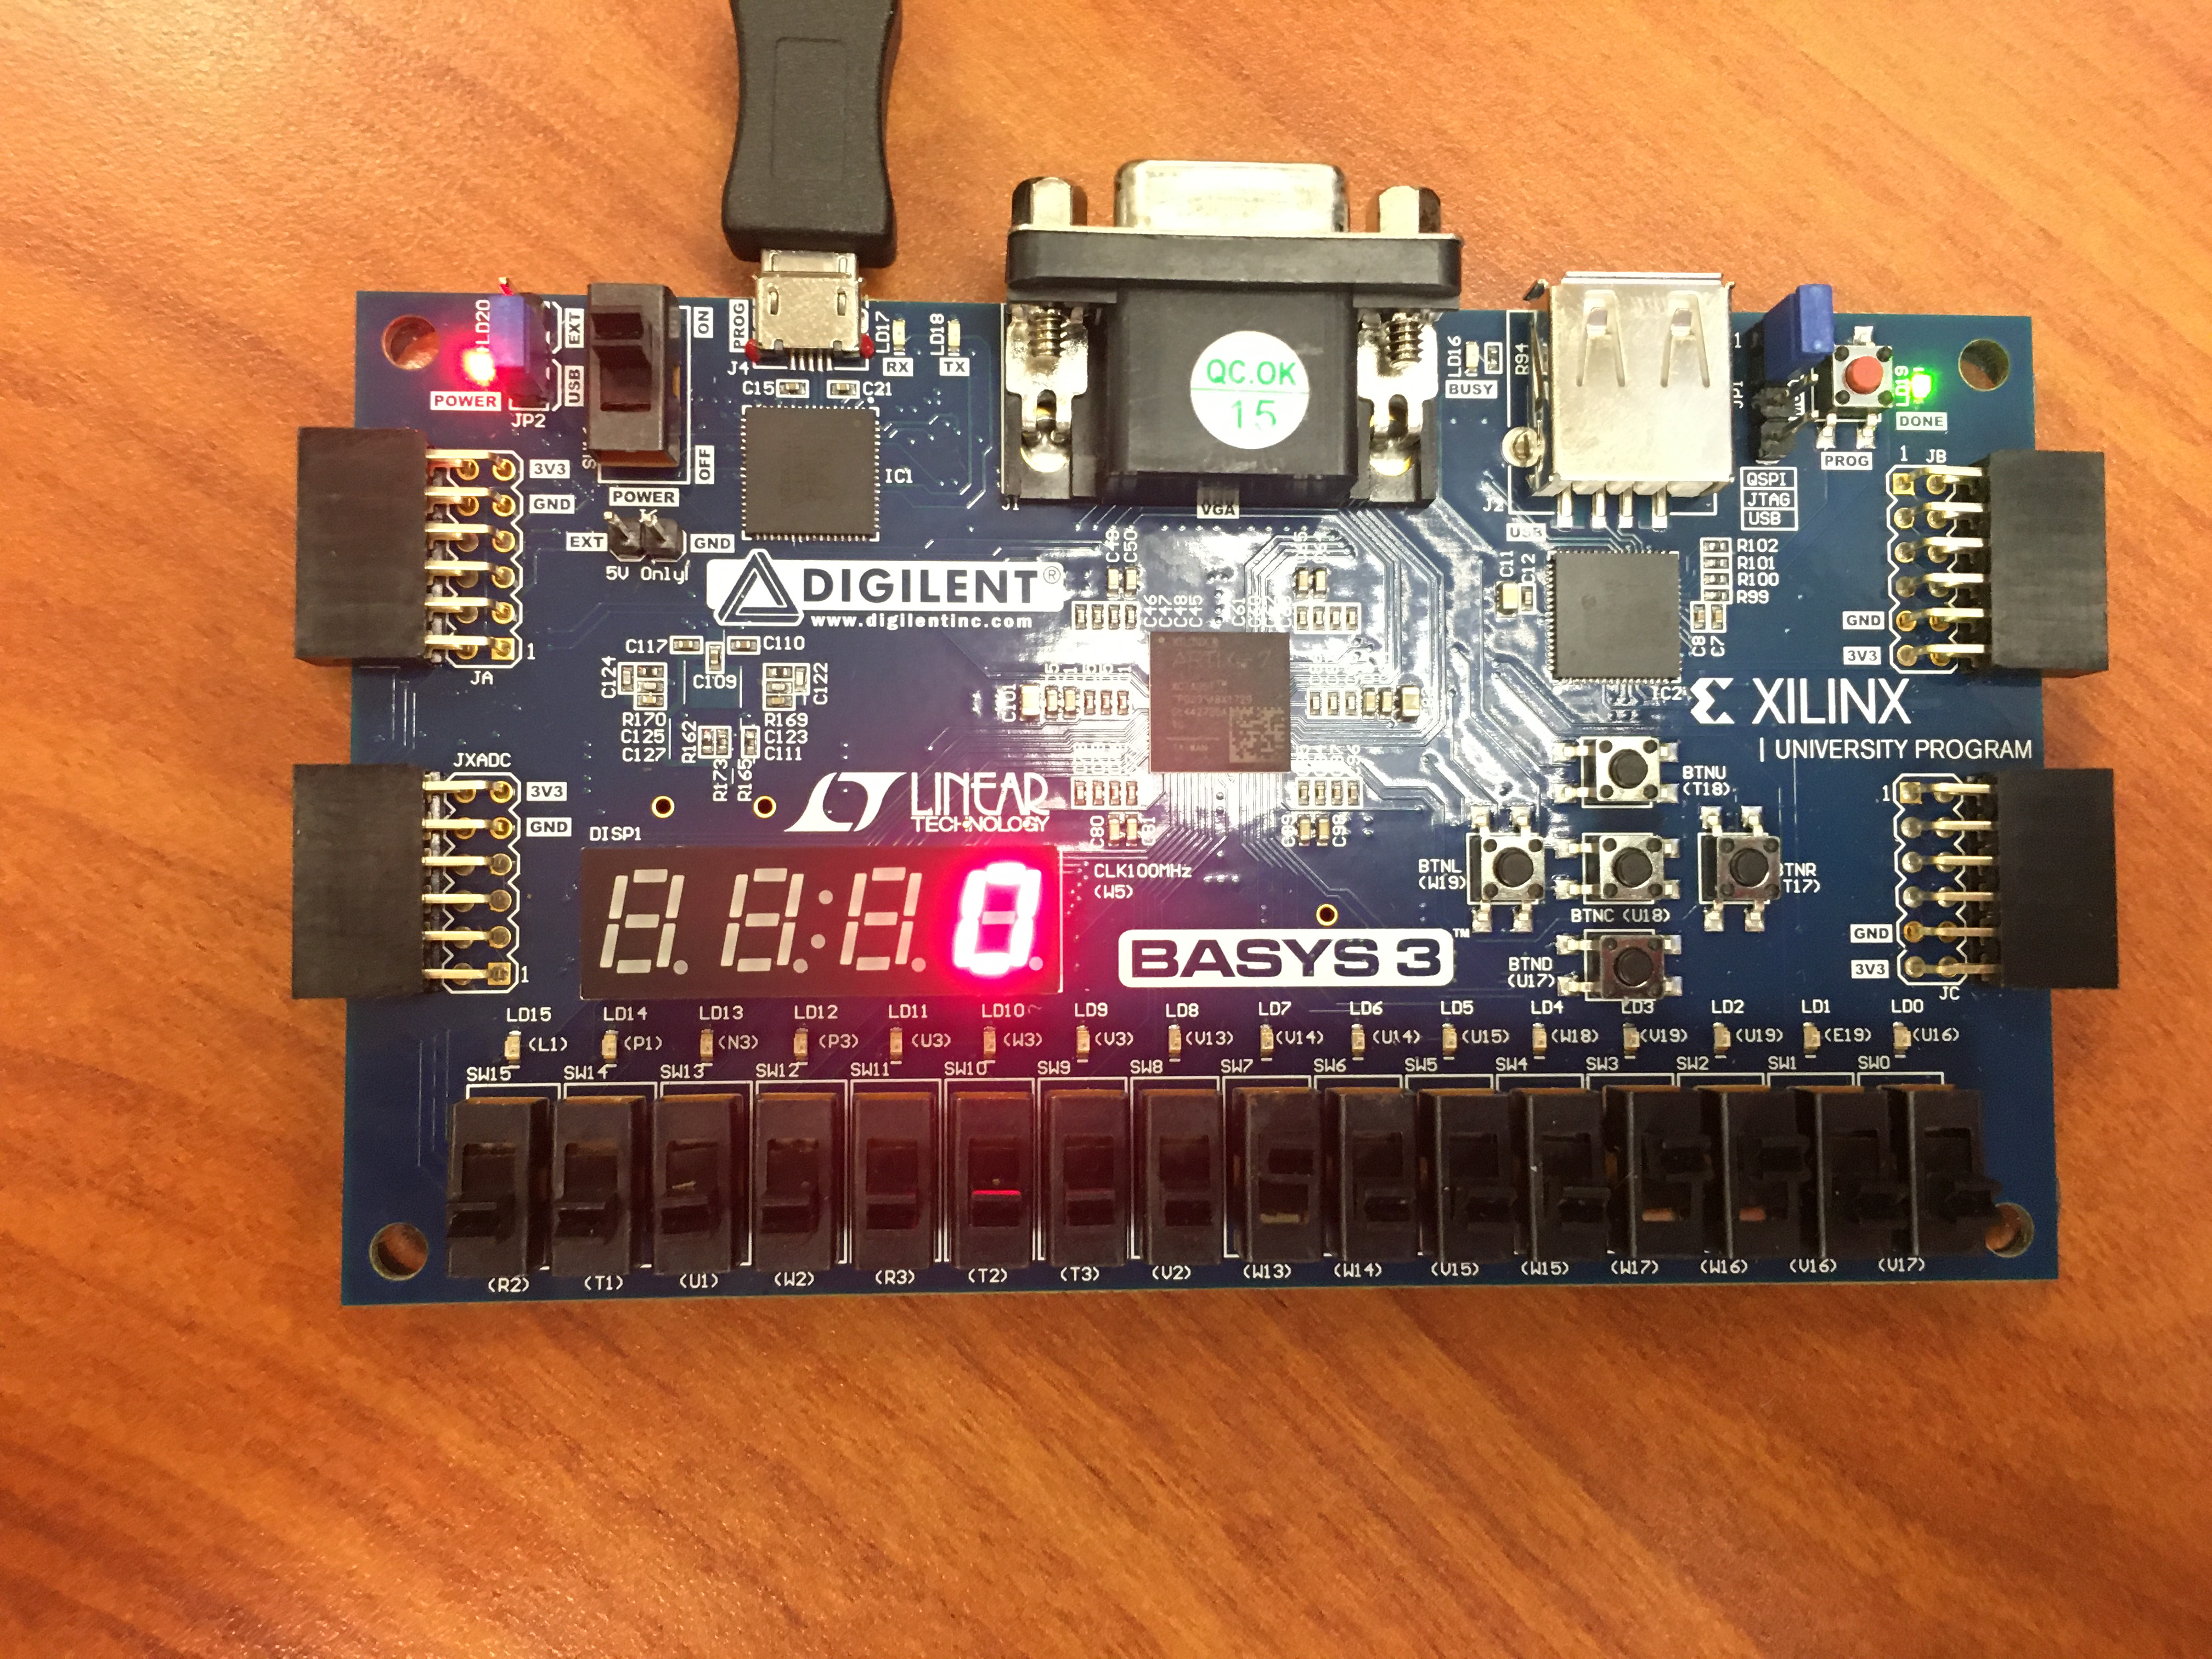
\includegraphics[width=12cm]{"board/step7}
	\caption{7th Operation}
\end{figure}
\begin{figure}[ht]
	\centering
	\includegraphics[width=12cm]{"board/step8"}
	\caption{8th Operation}
	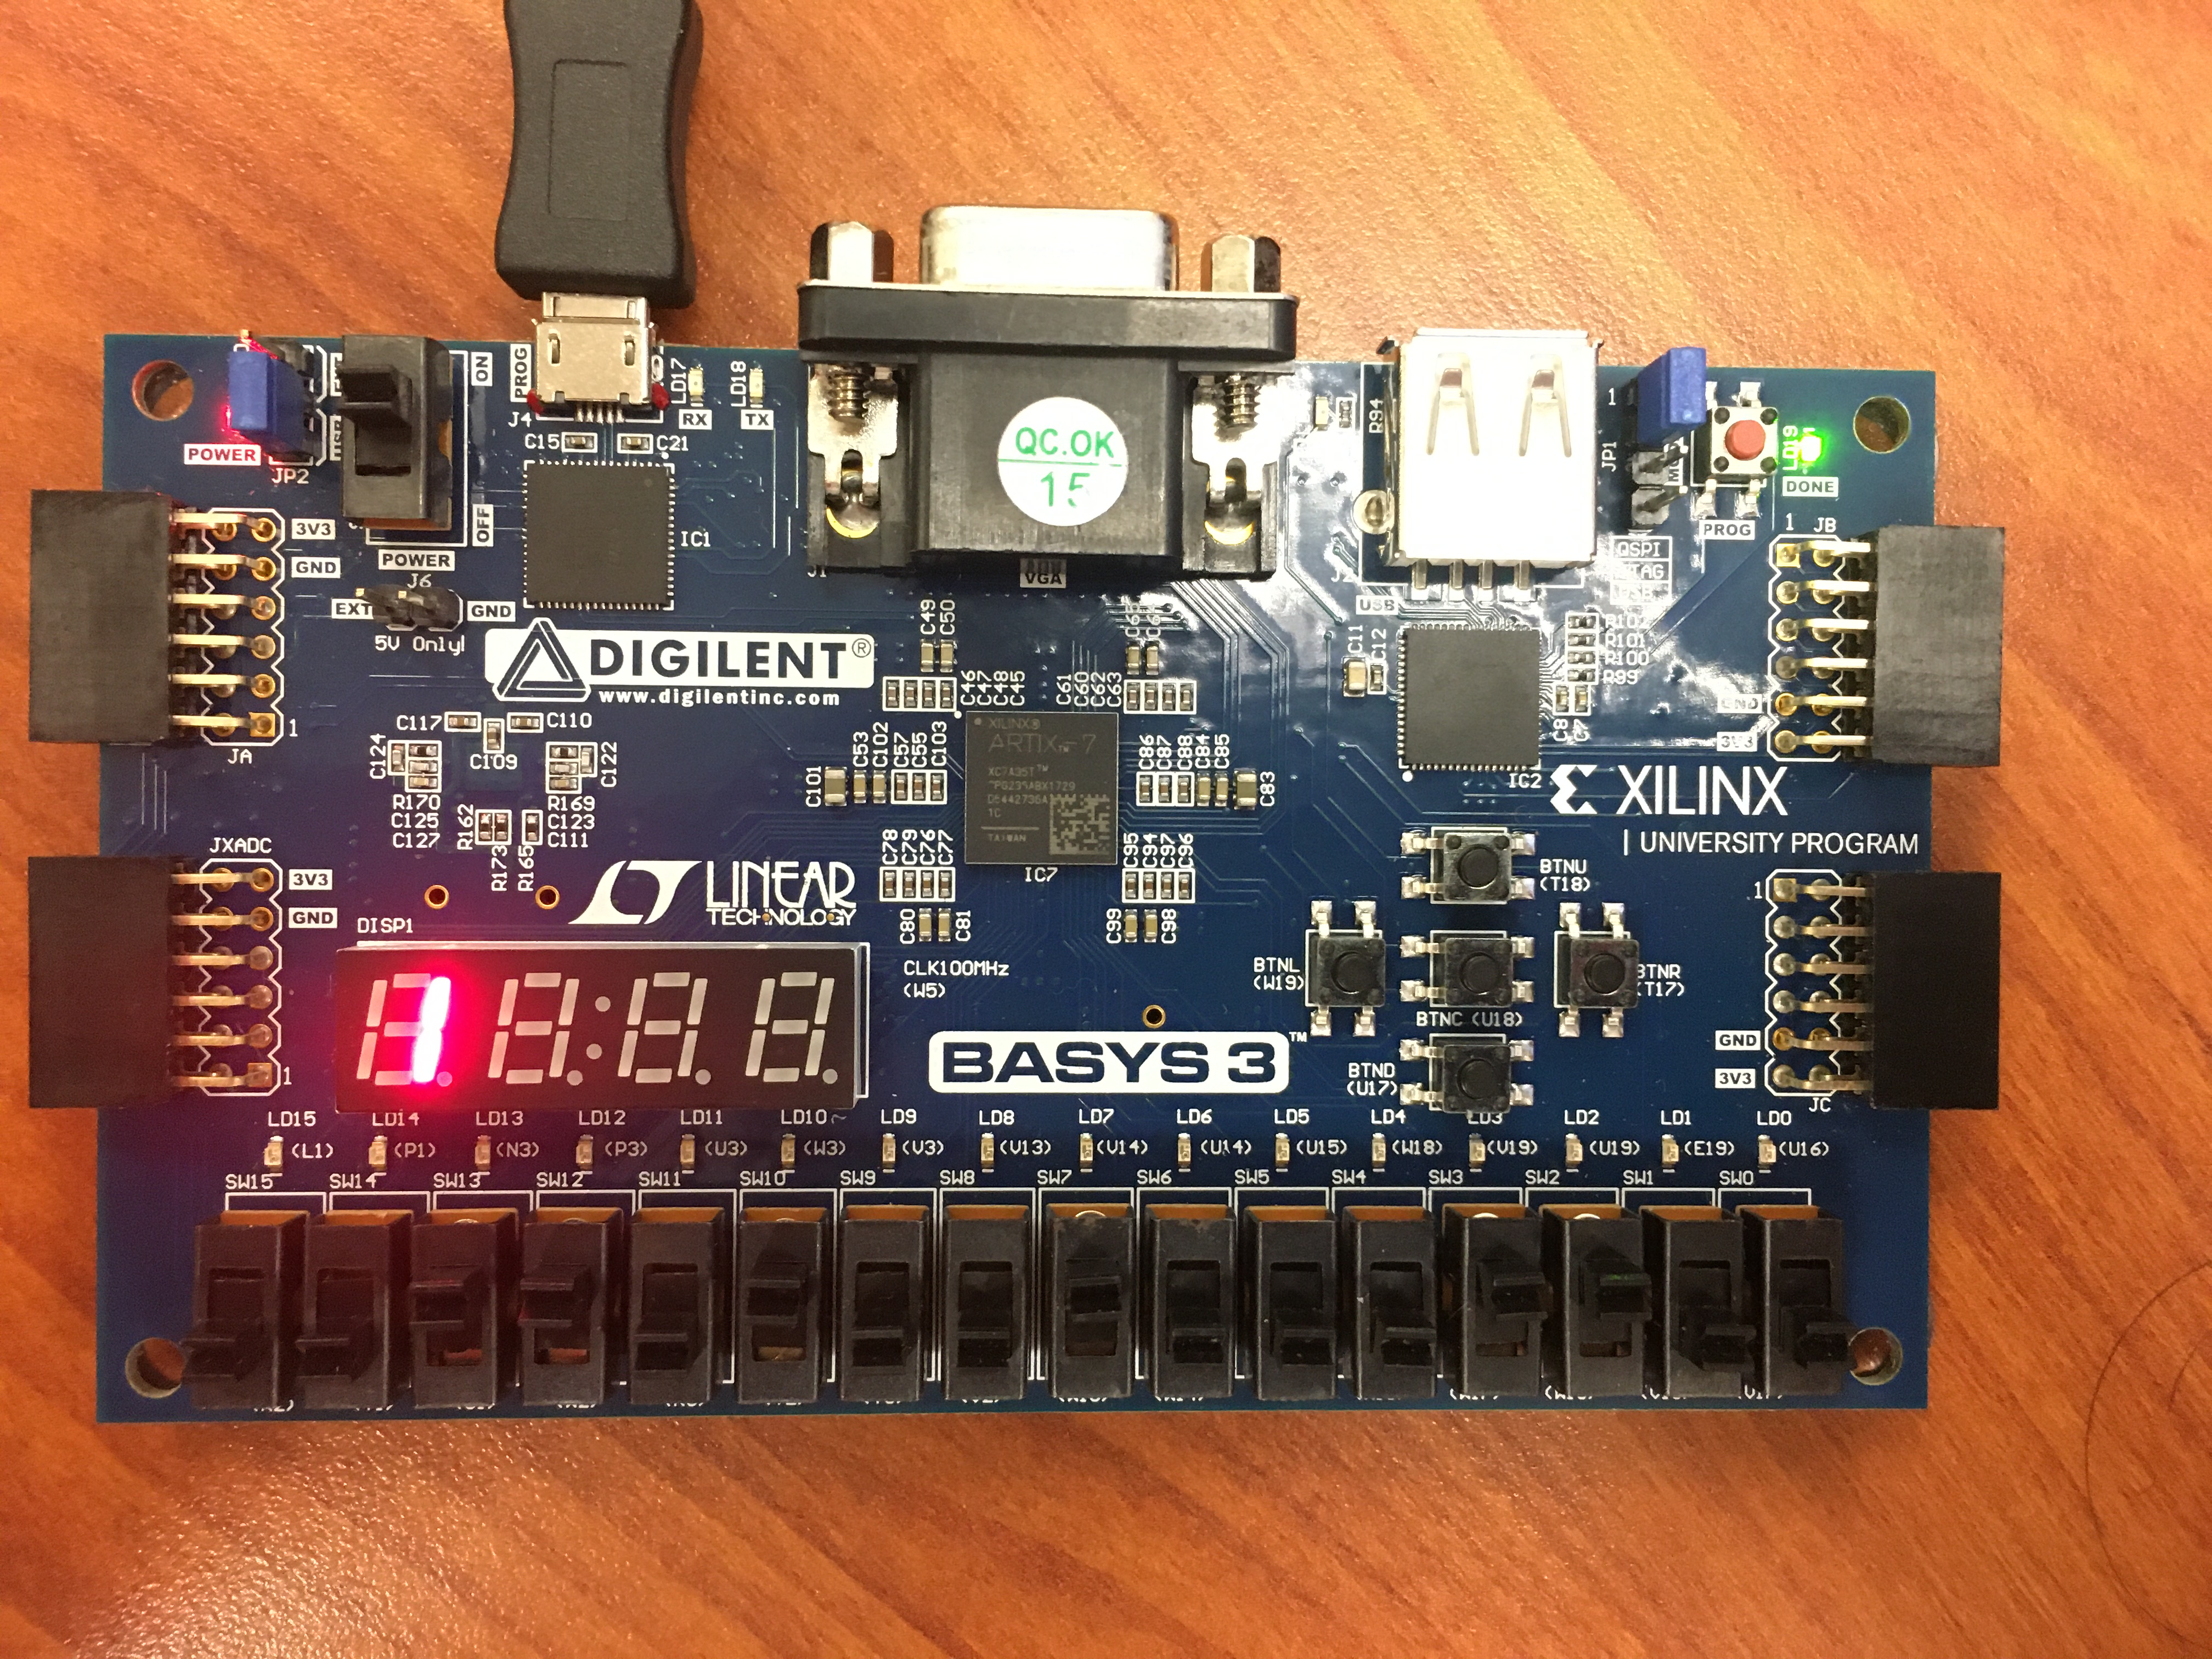
\includegraphics[width=12cm]{"board/step9}
	\caption{9th Operation}
\end{figure}
\begin{figure}[ht]
	\centering
	\includegraphics[width=12cm]{"board/step10"}
	\caption{10th Operation}
	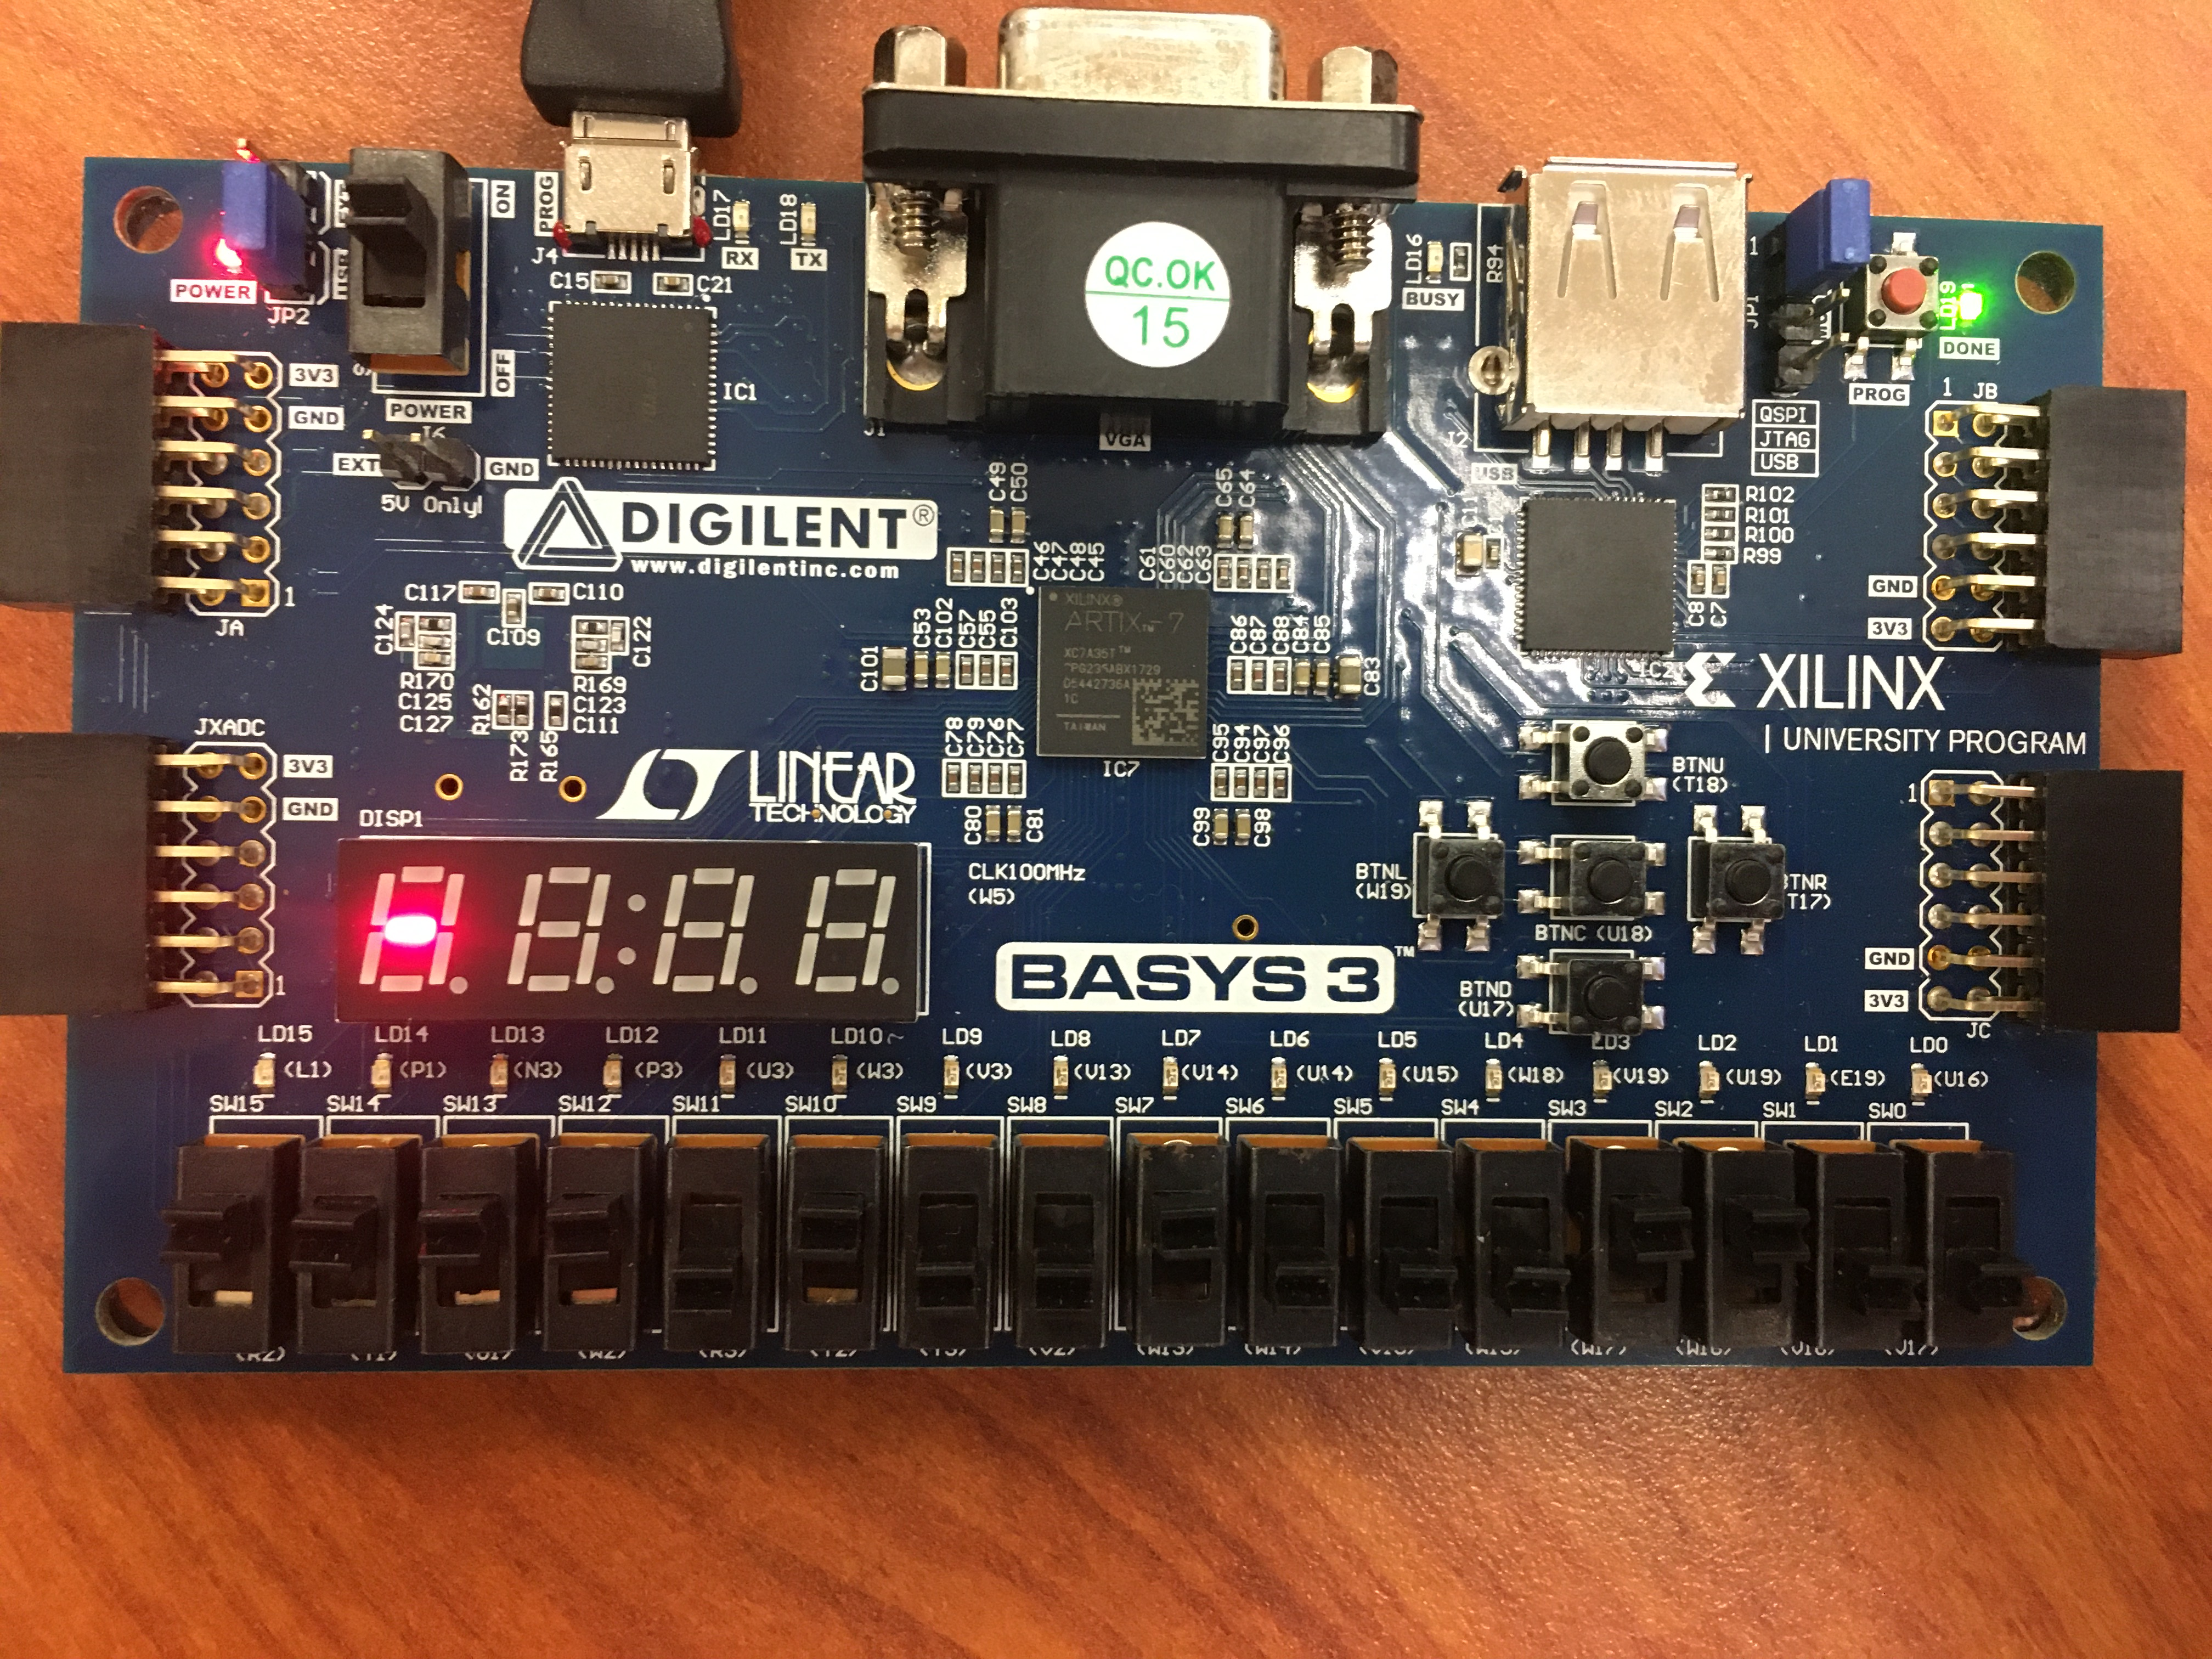
\includegraphics[width=12cm]{"board/step11}
	\caption{11th Operation}
\end{figure}

\begin{figure}[ht]
	\centering
	\includegraphics[width=12cm]{"simulation_results"}
	\caption{Simulation Results}
\end{figure}



%\section*{Questions}

\end{document}
